\Chapter{Módosító algoritmusok}

\Section{Az eloszlások távolságának mérése}

Az eloszlások ill. gyakoriságok távolságát több módon is mérhetjük.
Mivel nem cél a különböző metrikákkal kapott hibaértékek összehasonlítása, ezért lényegtelen hogy a mért és elvárt gyakoriságok vagy/és valószínűségek távolságát vizsgáljuk.
Ennek a hibának a mérésére a mért és elvárt értékek különbségéből kapható vektor normáival is megtörténhet:
\[
\vec{v} = \vec{e} - \vec{m},
\]
ahol az $\vec{e}$ az elvárt (\textit{expected}) és az $\vec{m}$ a mért (\textit{measured}) értékeket tartalmazza.

Az így kapott vektor 1-es normája által meghatározott érték megfelel a mért és elvárt adatok közötti abszolút különbségek összegével.
\[
\left\lVert\vec{v}\right\rVert_1 = \sum\limits_{i=1}^{n} |v_i|
\]
A 2--es norma a távolságok négyzetösszegének a gyökét adja vissza.
\[
\left\lVert\vec{v}\right\rVert_2 = \sqrt{\sum\limits_{i=1}^{n} |v_i|^2}
\]
A végtelen norma pedig a legnagyobb távolság abszolút értékét határozza meg.
\[
\left\lVert\vec{v}\right\rVert_\infty = \max\limits_{i=1}^{n} |v_i|
\]

Lehetséges ezeken kívül az átlagos négyzetes hibának (\textit{mean squared error, MSE}) számítása, amely nem sokban tér el a 2-es norma számításától.
\[
MSE(\vec{v}) = \frac{1}{n} \sum_{i=1}^{n}(v_i)^2
\]

Az eloszlások távolságának a mérésére a $\chi^2$-et szokták még alkalmazni, amellyel később meg lehet vizsgálni hogy milyen szignifikancia szinten egyezik meg az elvárt és mért értéksorozat.
\[
\chi^2=\sum_{i=1}^{n} \frac{(e_i - m_i)^2}{e_i}
\]

A fent említett metrikák közül az MSE-t valamint a $\chi^2$-et használják a leggyakrabban, ezért ezeket fogjuk összehasonlítani optimalizálás során.

Egy tetraéder optimalizálása során az alábbi értékeket mértük:
\begin{verbatim}
1 mse = 0.012605000000000002   chi2 = 309.3075
2 mse = 0.005730000000000002   chi2 = 133.22333333333333
3 mse = 0.004737500000000001   chi2 = 123.45833333333333
4 mse = 0.0024330000000000007  chi2 = 69.02083333333334
5 mse = 0.001435500000000001   chi2 = 33.730000000000004
6 mse = 0.0010555000000000004  chi2 = 16.908333333333335
7 mse = 0.00019650000000000003 chi2 = 3.2125
8 mse = 0.0010955000000000001  chi2 = 21.553333333333335
9 mse = 7.399999999999977e-05  chi2 = 1.0333333333333332
\end{verbatim}
Addig módosítottuk a testet, amíg a kapott MSE érték $10^{-4}$ allatti nem lett. A dobássorozatok mérete $N=1000$ volt, és a későbbi \ref{sect:facemodification} szakaszban mutatott heurisztikát használtuk.
Az értékek által meghatározott görbék alakra nagyon hasonlónak tűntek, ezért a legkisebb négyzetek módszerét alkalmazva összehasonlítjuk őket.
A számítások alapján $a_0 + a_1\cdot mse = \chi^2$, ahol $a_0 = -1.67216109, a_1 = 24742.3397$.
\begin{figure}[h!]
	\centering
	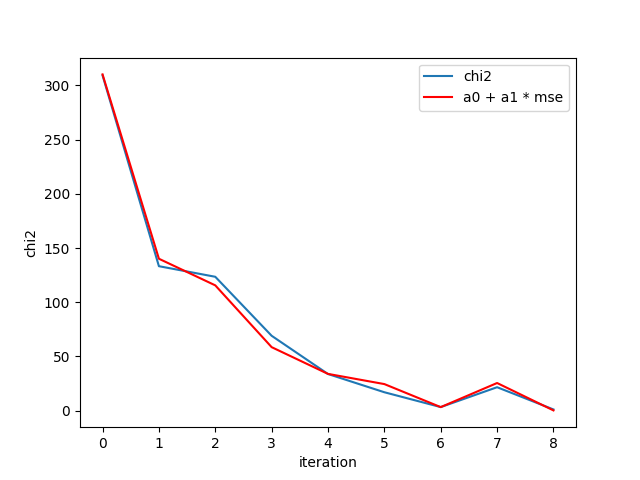
\includegraphics[scale=0.7]{images/mse_vs_chi2.png}
	\caption{A módosított MSE, és a $\chi^2$ értékek.}
	\label{fig:mse_vs_chi2}
\end{figure}
A \ref{fig:mse_vs_chi2} ábra mutatja, hogy a feltételezésünk igaz volt, a két érték konvergálása hasonló, emiatt nincs lényeges különbség aközött, hogy melyiket fogjuk használni.
A végső választás azért esett a $\chi^2$-re, mert így tudjuk folyamatosan nyomon követni, hogy egy adott szignifikancia szinten el tudjuk-e fogadni a módosított test által adott gyakoriságokat.

\Section{Egyetlen pont mozgatása}
\label{sect:randmodification}

Ez a módszer a testet úgy módosítja, hogy mindig egy véletlenszerűen választott csúcspontját egy egység hosszúságú vektorral odébb helyezi.
A vektort a \ref{subs:randompoint} szakaszban említett módszerrel generáljuk.
Amennyiben a módosított test dobássorozata alapján kapott gyakoriságok jobbak mint az eredeti testé, az új testen végezzük el ugyan ezt a lépést, egyébként a módosítatlan testen.
\begin{figure}[h!]
	\centering
	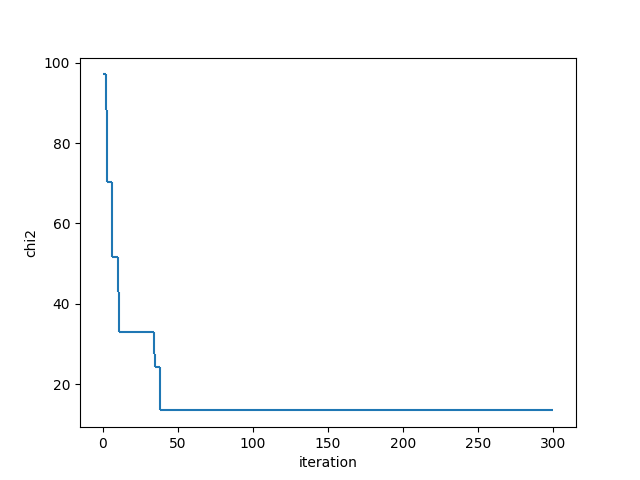
\includegraphics[scale=0.7]{images/randmodify_chi2.png}
	\caption{Egyetlen pont elmozdításával kapott test módosítása közben mért legjobb $\chi^2$ értékek.}
	\label{fig:randmodify_chi2}
\end{figure}
A \ref{fig:randmodify_chi2} grafikon egy tetraéder módosítása közben mért értékeket mutatja.
Az elvárt eloszlás [0.1, 0.2, 0.3, 0.4], leállás feltételéhez az iterációk száma $300$, a dobás sorozatok mérete pedig $N=200$.
A végén kapott testtel egy $N=1000$ méretű dobássorozatnál a $\chi^2$ értéke $298.78$.
Láthatjuk hogy az így kapott érték túl nagy ahhoz hogy a testet $\alpha = 0.05$ szignifikancia szinten el tudjuk fogadni.
Ebből arra tudunk következtetni, hogy a rossz módosítást a kis méretű dobássorozaton pontatlanul mért értékek miatt helyes módosításként kezelte.
Az így elmenett hibás állapotokból gyakran nem tudja az eljárás korrigálni jó irányba a testet.

Ez a módszer a véletlenszerű módosítások miatt nem tud konzisztensen egy megadott hibaküszöbhöz konvergálni, ezért futási paraméternek a módosító iterációk számát kell megadni hibaérték helyett.
Ez abból következik, hogy nem veszi figyelembe az elkövetett hibás módosításokat és nem von le következtetéseket a mért gyakoriságokból.

Mivel fix hosszúságú vektorral módosítjuk a testet és sosem lépünk vissza rosszabb hibaértéket adó testhez, így előfordulgat, hogy nem tudunk egy bizonyos hibaérték alá menni az optimalizálás során, mert a pontok egységsugarú környezetében található az optimális pozíciója.
Ezt úgy tudjuk kijavítani, hogy az iterációszám és a hibaértéktől függően csökkentjük a módosító vektorok hosszát.

A fent említett okok miatt érdemesebb más heurisztikával optimalizálni a testeket.

\Section{Oldallapok méretének módosítása}
\label{sect:facemodification}

Ez az algoritmus a csúcspontokat aszerint mozgatja, hogy oldallapokra nézve az elvárt és mért valószínűség hogyan viszonyul egymáshoz.
Ha az adott oldallap előfordulásán növelni szeretnénk akkor a csúcsokat lap súlypontjából kifelé mutató egység hosszúságú vektorokkal mozdítjuk el, egyébként a csúcsokat a súlypont felé mozgatjuk.

A \ref{fig:facemodification} ábrán látható kék vektorok felelnek az oldallap növeléséért, a vörösek pedig annak csökkentéséért.

\begin{figure}[h!]
	\centering
	\begin{tikzpicture}
		\node [label={[shift={(-0.2,-0.1)}]$C$},inner sep=0] (C) at (4,3) {};
		\node [label={[shift={(-0.2,0)}]$P_1$},inner sep=0] (P1) at (0,0) {};
		\node [label={[shift={(0.3,-0.2)}]$P_2$},inner sep=0] (P2) at (5,7) {};
		\node [label={[shift={(0.2,0)}]$P_3$},inner sep=0](P3) at (7,2) {};
		\draw (P1) -- (P2) -- (P3) -- (P1);
		\draw [dashed] (C) -- (P1);
		\draw [dashed] (C) -- (P2);
		\draw [dashed] (C) -- (P3);
		\node [inner sep=0] (out1) at (-0.8,-0.6) {};
		\node [inner sep=0] (out2) at (5.24,7.97) {};
		\node [inner sep=0] (out3) at (7.95,1.68) {};
		\draw [->, draw=blue] (P1) -- (out1);
		\draw [->, draw=blue] (P2) -- (out2);
		\draw [->, draw=blue] (P3) -- (out3);
		\draw [dotted] (out1) -- (out2) -- (out3) -- (out1);
		\node [inner sep=0] (in1) at (0.8,0.6) {};
		\node [inner sep=0] (in2) at (4.76,6.03) {};
		\node [inner sep=0] (in3) at (6.05,2.32) {};
		\draw [->, draw=red] (P1) -- (in1);
		\draw [->, draw=red] (P2) -- (in2);
		\draw [->, draw=red] (P3) -- (in3);
		\draw [dotted] (in1) -- (in2) -- (in3) -- (in1);
	\end{tikzpicture}
	\caption{Oldallap méretének változtatása egység hosszúságú vektorral.}
	\label{fig:facemodification}
\end{figure}
\begin{figure}[h!]
	\centering
	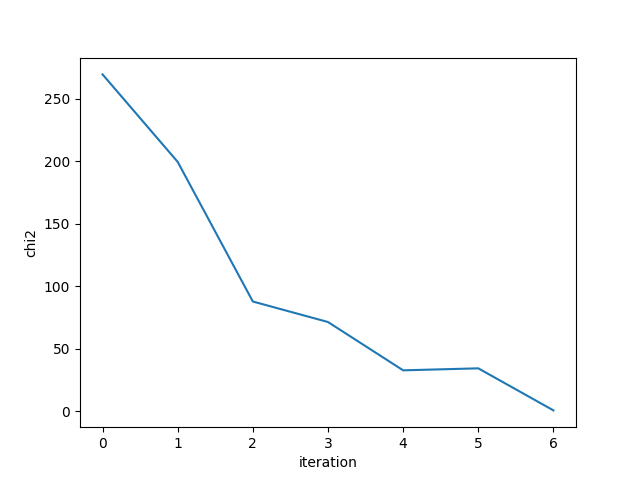
\includegraphics[scale=0.7]{images/facemodify_chi2.png}
	\caption{Az oldallapok méretének módosításával mért $\chi^2$ értékek az iterációk függvényében.}
	\label{fig:facemodify_chi2}
\end{figure}

A \ref{fig:facemodify_chi2} grafikonon látható egy tetraéder módosítása közben kapott átlagos négyzetes hibák.
A várt eloszlás [0.1, 0.2, 0.3, 0.4], a dobássorozatok mérete $N=1000$, leállási feltétel pedig a $\chi^2 < 2.5$.
A végén kapott test $1000$ dobásra nézve $\chi^2 = 3.5983$ értéket adott.
Ez amiatt lehetséges, hogy a leállásnál mért értékek pontatlanság miatt közelebb voltak a várt értékekhez.
Ha kellően alacsonyra állítjuk be a küszöbértéket, akkor az ilyen hibák mellett is tudunk olyan testet kapni, amelyet egy adott $\alpha$ szignifikancia szinten el tudunk fogadni.

A \ref{subs:randompoint} szakaszban bemutatott módszerhez képest látványosan gyorsabb, és egyértelműen konvergál az elvárt eloszláshoz.
Mivel az algoritmus az aktuálisan mért eloszlásokhoz képest módosítja a lapok méretét, így az esetlegesen elkövetett hibákat folyamatosan tudja javítani, valamint mivel sokkal gyorsabban konvergál, így nyugodtan adhatunk meg nagyobb dobásméretet, amellyel tovább tudjuk csökkenteni az esetleges fals méréseket.

\Section{Módosítás az arányok figyelembe vételével}
\label{sect:ratiomodification}

Ez a folyamat szinte teljes mértékben megegyezik az előző pontban leírt metódushoz.
Az egyetlen lényeges különbség annyi, hogy az oldallapokat a gyorsabb konvergencia miatt nem egység hosszú vektorokkal módosítjuk.
A módosító vektorok hossza függ az oldallapokhoz mért és elvárt valószínűségek különbségétől, hogy a nagyobb eltérések esetében drasztikusabban tudjuk az oldallapokat módosítani.
Olyan eset is előfordulhat, hogy az oldallap ideális méretének eléréséhez az oldallapot fél egység hossz vektorokkal kéne növelnünk, és ezt a méretet a \ref{sect:facemodification} szakaszban leírt függvénnyel nem tudjuk elérni.

Az algoritmus a módosító vektorok hosszát az oldallapokhoz tartozó várt és mért valószínűségek különbségével határozza meg.
Ezt a különbséget egy $\lambda$ konstanssal megszorozva tudunk a konvergencia sebességén módosítani.
\begin{figure}[h!]
	\centering
	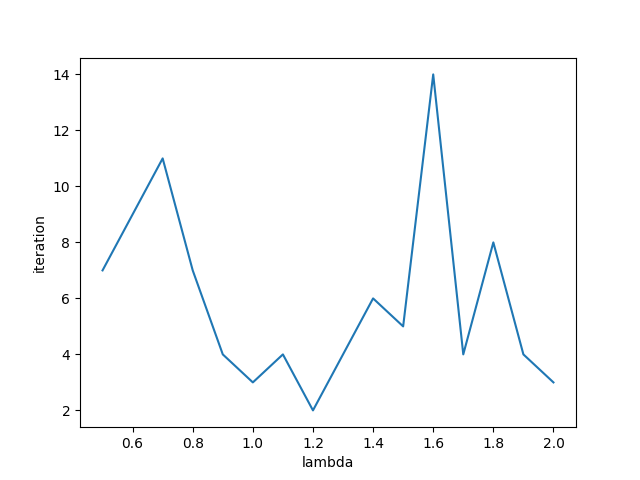
\includegraphics[scale=0.7]{images/lambdatest.png}
	\caption{Az algoritmus futásához szükséges iterációk $\lambda$ függvényében.}
	\label{fig:lambda}
\end{figure}

A \ref{fig:lambda} grafikonon látható egy tetraéder módosításához szükséges iteráció számok az egyes $\lambda$ értékekhez.
Látható hogy nem tudunk egyértelműen meghatározni ez alapján egy egyértelmű minimumot.
Hogy ezt meg tudjuk tenni minden $\lambda$ értékhez több dobássorozatot kéne csinálnunk, és az így mért iterációszámokat kéne átlagolnunk.
Az egyes módosítások hossza nagyban függ a test alakjától, a várt eloszlástól, az elő mérés pontosságától, valamint a $\lambda$ értéktől.
Minden testre és azokhoz tartozó eloszlásra nézve a $\lambda$ meghatározása sokkal több időt vesz igénybe, mint ha végig egy adott konstans értékkel számolnánk.
Emiatt az optimalizálásnál $\lambda = 1$ értékkel fogunk számolni.